\documentclass[11pt]{article}
\usepackage{geometry}                % See geometry.pdf to learn the layout options. There are lots.
\geometry{letterpaper}                   % ... or a4paper or a5paper or ... 
%\geometry{landscape}                % Activate for for rotated page geometry
%\usepackage[parfill]{parskip}    % Activate to begin paragraphs with an empty line rather than an indent
\usepackage{graphicx}
\usepackage{amssymb}
\usepackage{epstopdf}
\usepackage[usenames,dvipsnames]{color}
\DeclareGraphicsRule{.tif}{png}{.png}{`convert #1 `dirname #1`/`basename #1 .tif`.png}

\title{User's guide for cvis - a program to visualize networks using clusters}
%\date{}                                           % Activate to display a given date or no date

\begin{document}
\maketitle
%\section{}
%\subsection{}



\section{Get Started}

The program comes along with a file called \textbf{compile\_all.sh}.

Type:

{ \textbf{./compile.sh} }

from a Unix (MAC) terminal. If you are using Windows, you could still run
the program by installing MinGW
(Minimalist GNU for Windows, {\tt http://www.mingw.org/}).
If you see something like \textbf{./compile.sh: Permission denied}, type:

\textbf{chmod 744 compile.sh} 

which makes the script executable and try again with:

\textbf{./compile.sh}. 

Now try:

{ \textbf{./cvis\_undir -f network.dat -folder network.dat\_oslo\_files} }




\section{Output files}

If you open the folder \textbf{network.dat\_cvis }, you will see a few files:

\begin{itemize}
  \item \textbf{cvis\_0.gdf} is the most important: it can be opened using gephi ({\tt http://gephi.org/}). You should see two clusters of nodes with the same colors, one white (not assigned) node and one bright overlapping node. 
  \item  \textbf{cvis\_1.gdf} will visualize the same network where nodes belonging to the lowest level are aggregated.
  \item \textbf{node\_memberships.dat} reports the number of clusters each node belongs for the different hierarchical levels (from fine levels to coarse ones)
  \item \textbf{modules\_1.dat} reports the nodes contained in each module of the first hierarchical level. 
\end{itemize}


\begin{figure}[h!]
\begin{center}
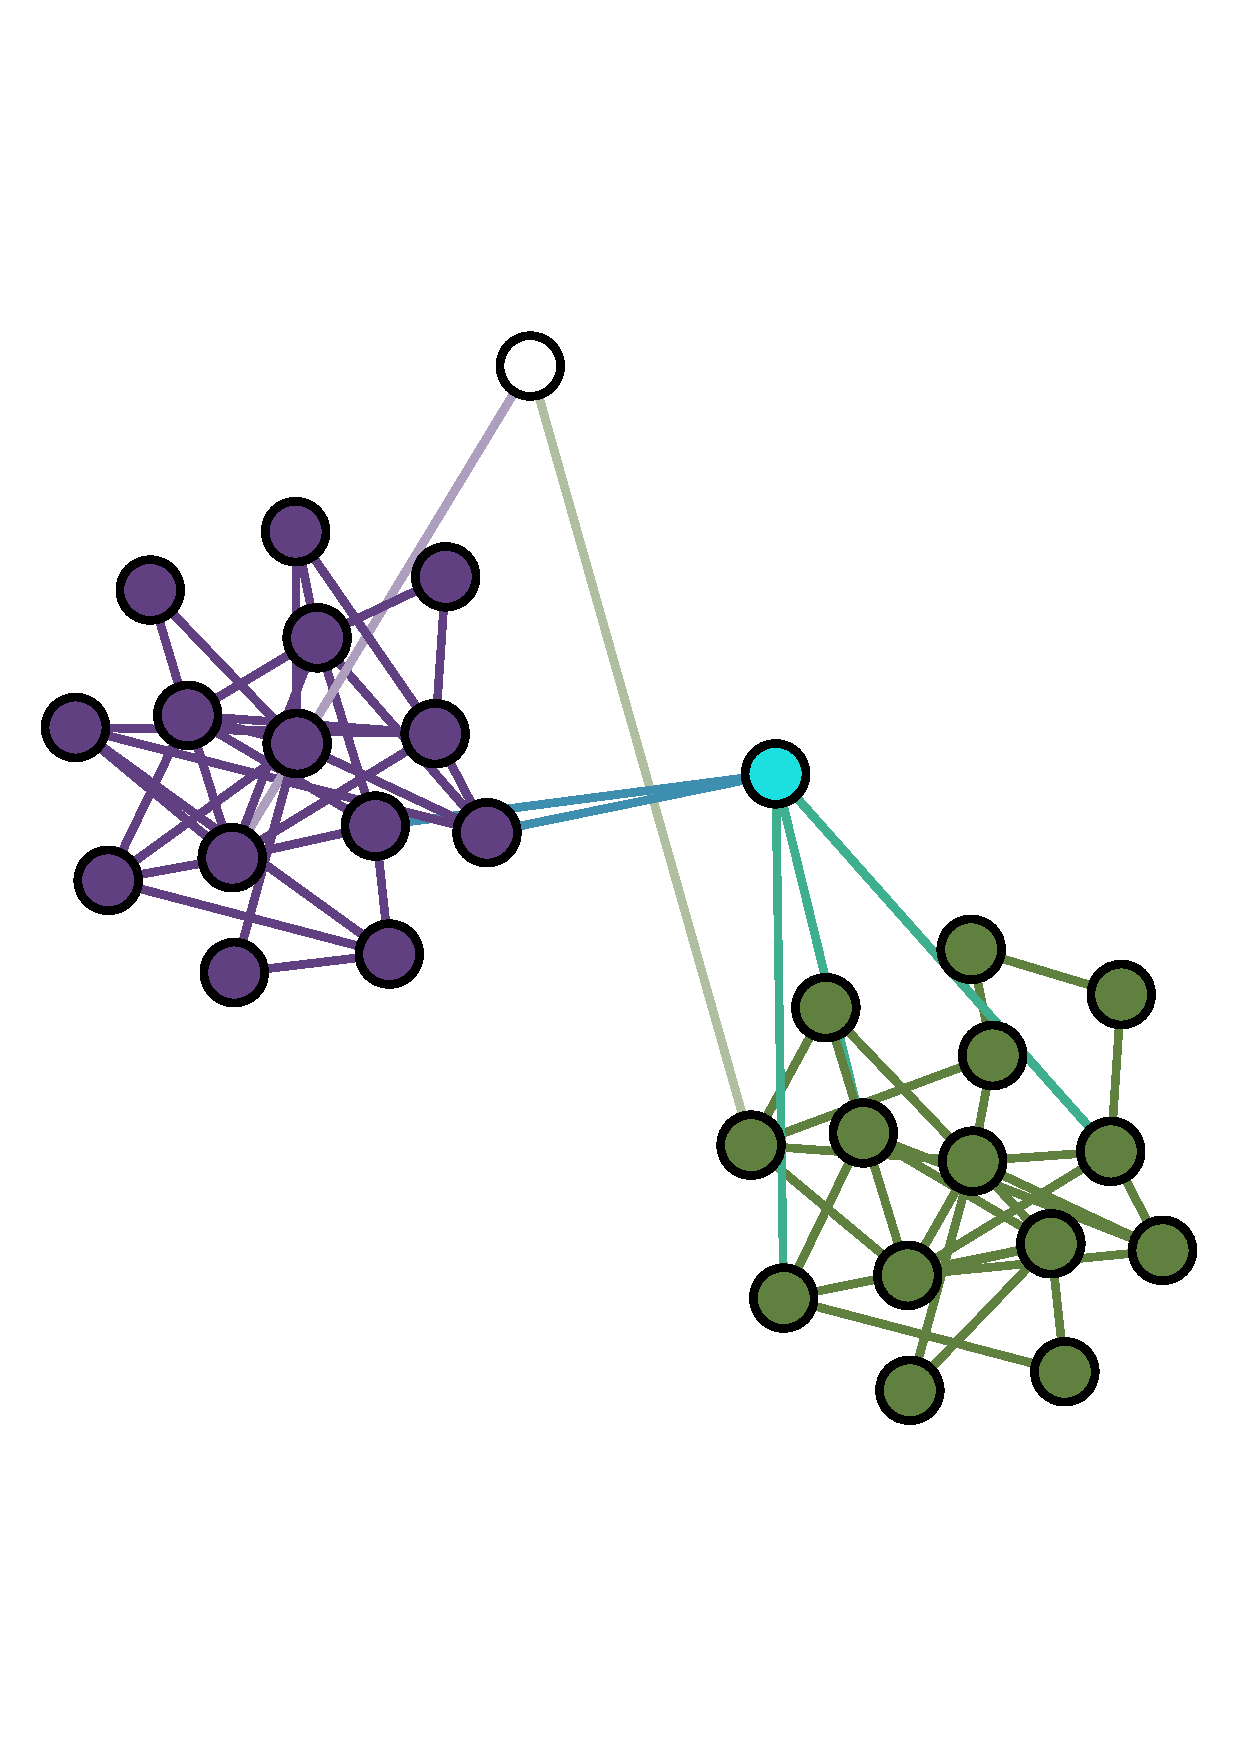
\includegraphics[width=2.5in]{network.pdf}
\caption{Visualization of  \textbf{network.dat\_cvis/cvis\_0.gdf} }
\end{center}
\end{figure}




\section{Input files and Options}

To run the program, you first need to run a clustering algorithm and find the modules you want to visualize. The modules can be hierarchical and overlapping. 

Choose between \textbf{cvis\_undir} (undirected networks) and \textbf{cvis\_dir} (directed networks).
Then, you need to select the network and the partitions:


\begin{enumerate}
  \item \textbf{-f network\_file}: network\_file is expected to contain the edge list, with possible weights.   
  \item \textbf{-folder network\_file\_folder}:  network\_file\_folder is the folder which contains the partitions. It is expected to contain a file called \textbf{tp},  which is the set of (overlapping) modules at the lowest hierarchical level (each row corresponds to a cluster). The higher hierarchical modules are specified in files \textbf{short\_tp1}, {\bf short\_tp2} \dots. \textbf{short\_tp1} gives the second hierarchical level modules: the ids refers to the modules written in \textbf{tp} indexed in order of appearance (for instance, a row like $0\,\,1\,\,2$ means that the first, second and third modules of \textbf{tp} are put together at this level). This folder is formatted as the output given by OSLOM $[1]$
   \item \textbf{-tree network\_tree}:  network\_tree is a unique file which specifies all the partitions. This option can be used instead of  option  \textbf{-folder}. Here, each row contains the module assignments from the coarse to the fine level. The last word is the node id. This is the same format given by hierarchical infomap [2]. 
\end{enumerate}



\section{Other Options}

\begin{enumerate}
  \item \textbf{-labels filename}: filename contains the node labels, which are strings. The format of the file is: string node\_id. For an example, look at file \textbf{labels\_nodeid.dat}. Please note that the node labels should not contain characters like \textbf{, -} or \textbf{"}, otherwise gephi gets confused. 
  \item \textbf{-opt U [0, 5]}: U is an optimization parameter. Higher values of U take more time and lead to better results. Default value is 2.  
    \item \textbf{-gap U}: this is to decide how far the modules should be. Default is 1.4. Reasonable values should be between 1 and 2.
      \item \textbf{-singlets U}: this is a parameter used to locate singletons (clusters with one only node). Default is 0.5 (must be U$> 0$). Bigger values create a layout where singletons occupy more space (more CPU consuming).
 \item \textbf{-seed U}: seed for the random number generator. Default value is read from file \textbf{time\_seed.dat}, and is automatically increased every time that file is opened.
\end{enumerate}


\section{References}



\begin{enumerate}

  \item \textbf{oslom}: { \tt http://www.oslom.org/}
  \item \textbf{hierarchical infomap}: {\tt http://www.tp.umu.se/$\sim$rosvall/code.html}
\end{enumerate}






\end{document}





         
